\documentclass{article}
\usepackage[utf8]{inputenc} 
\usepackage{graphicx} 
\usepackage{float} 

\title{Data Set}
\author{Nikunj Gupta}
\date{August 2018}

\begin{document}

\maketitle 

\section{Data Set information} 
It is a transnational data set which contains all the transactions occurring between 01/12/2010 and 09/12/2011 for a UK-based and registered non-store online retail.The company mainly sells unique all-occasion gifts. Many customers of the company are wholesalers. \newline 

\begin{itemize}
	\item Data Set Characteristics: Multivariate, Sequential, Time-Series
    \item Number of Instances: 541909 
    \item Attribute Characteristics: Integer, Real
    \item Number of Attributes: 8
\end{itemize}

\section{Attributes} 

\subsection{InvoiceNo} 
\textbf{Invoice number. }\newline 
Nominal, a 6-digit integral number uniquely assigned to each transaction. If this code starts with letter 'c', it indicates a cancellation. \newline 
Thoughts: Can be used to segregate orders. Considering a set of items as a single order.  

\subsection{StockCode} 
\textbf{StockCode } \newline 
Product (item) code. Nominal, a 5-digit integral number uniquely assigned to each distinct product. \newline 
Thoughts: Itemtype. 

\subsection{Description} 
Product (item) name. Nominal.
Thoughts: Names are too specific. Can be reduced to some common form. Other data preprocessing can also be done here. (Actually, Stock codes are enough for the missing values here.) 

\subsection{Quantity} 
The quantities of each product (item) per transaction. Numeric. \newline 
Thoughts: Can used to figure out the general demand amount per transaction. 

\subsection{InvoiceDate} 
Invoice Date and time. Numeric, the day and time when each transaction was generated. \newline 
Thoughts: The data is for a period of 1 year. So, only seasonal demands can be forecasted. 

\subsection{UnitPrice}
Unit price. Numeric, Product price per unit in sterling.
Thoughts: ItemSize would have been more useful perhaps. 

\subsection{CustomerID} 
Customer number. Nominal, a 5-digit integral number uniquely assigned to each customer. \newline 
Thoughts: Can be useful if we want to do Collaborative Filtering (Recommendation Systems). 

\subsection{Country} 
Country name. Nominal, the name of the country where each customer resides. 
Thoughts: Can be used to when we have many warehouses spread across a country/continent and we want our RL agent to figure out individual demands of these locations and accordingly manage the supply and placement of products. 


\section{Data Visualization} 
\subsection{Unique Elements} 
The following are the number of unique elements present in the dataset. For example, we have 4212 different products (Description) and 38 unique countries' data. 
\begin{figure}[H]
	%\hspace{-4.0cm}
	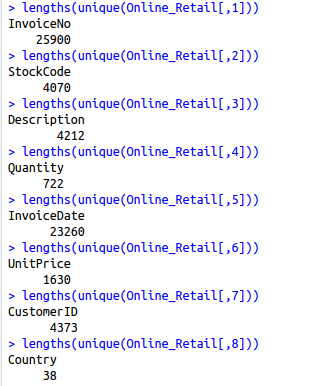
\includegraphics[width=6cm]{da/unique.png} 
	\centering 
\end{figure} 

\subsection{Country vs Quantity/InvoiceNo} 
This plot shows that UK has the most number of items ordered over the year. Here, the country attribute probably can be dropped and all products could be considered from the same place. 

\begin{figure}[h]
	%\hspace{-3.0cm}
	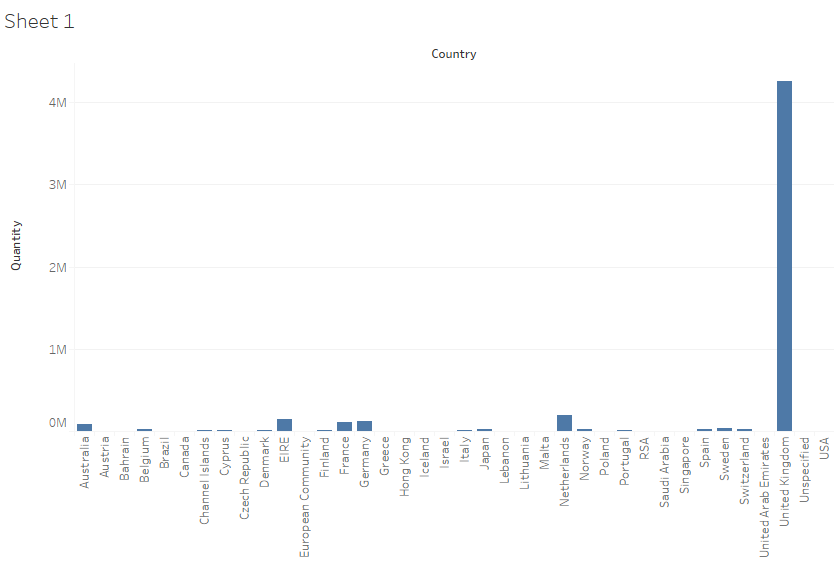
\includegraphics[width=13.5cm]{da/Sheet_1.png} 
	\centering 
\end{figure} 
\begin{figure}[h]
	%\hspace{-3.0cm}
	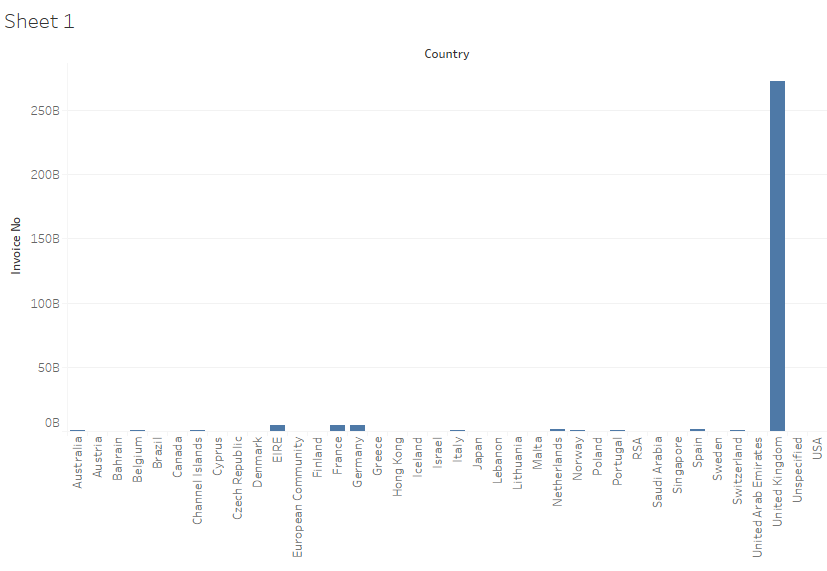
\includegraphics[width=13.5cm]{da/Sheet_2.png} 
	\centering 
\end{figure} 

\subsection{CustomerID vs Quantity } 
\begin{figure}[H]
	%\hspace{-3.0cm}
	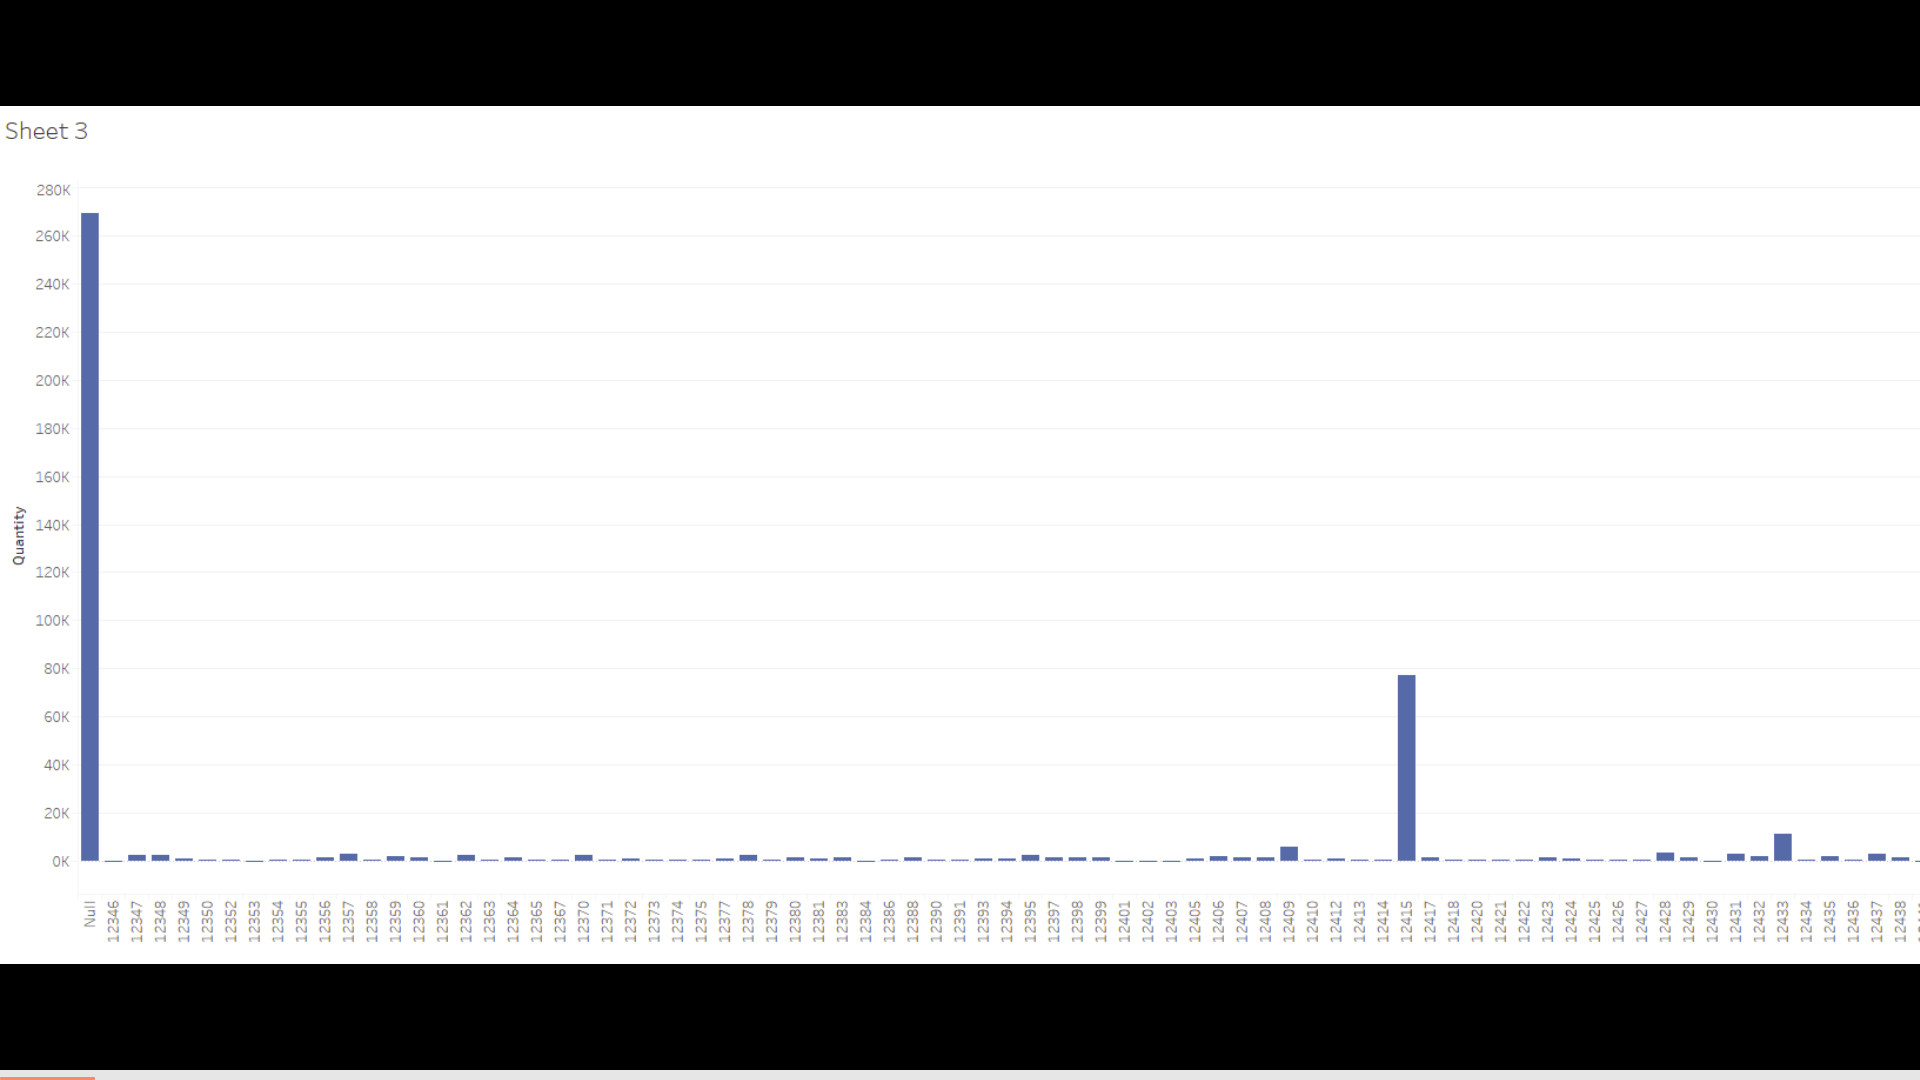
\includegraphics[width=13.5cm]{da/customerID.png} 
	%\centering 
	\end{figure} 

Majority of the CustomerIDs were NULL. So, we must omit this attribute. 

\subsection{Description vs Quantity} 
\begin{figure}[H]
	\hspace{-3.0cm}
	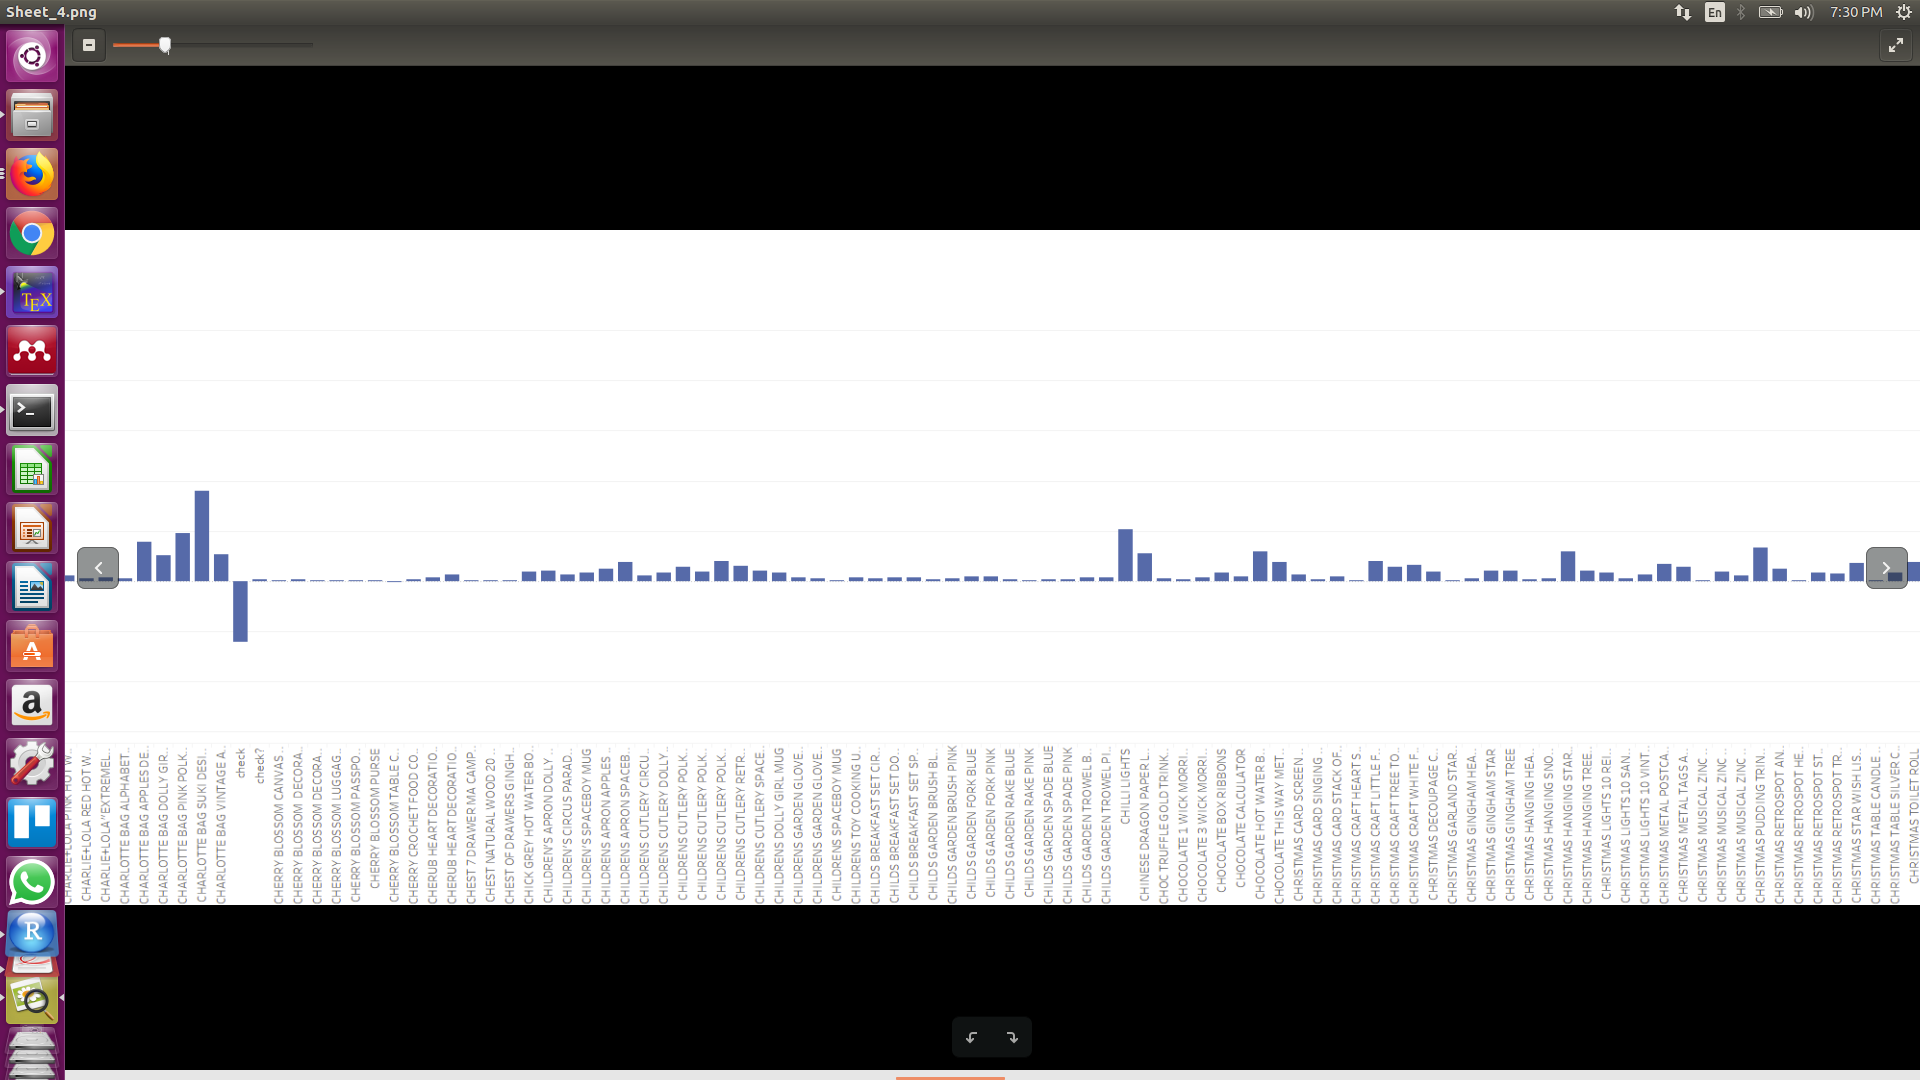
\includegraphics[width=18.5cm]{da/description.png} 	 
	\end{figure} 

This is a snapshot of some of the 4000+ products. Point to be noticed here is that some prodcuts have negative quantity here. The data needs preprocessing. 

\subsection{Negative Quantity} 

\begin{figure}[H]
	\hspace{-3.0cm}
	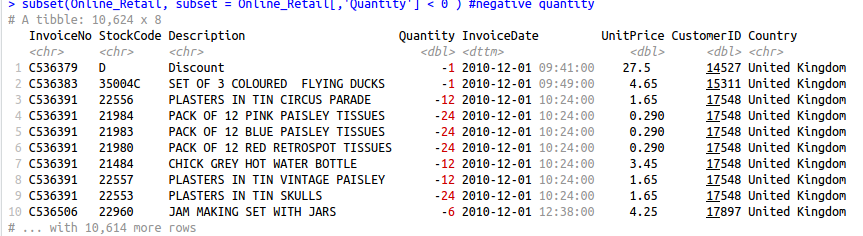
\includegraphics[width=18.5cm]{da/negative_quantity.png} 
	%\centering 
	\end{figure} 


\end{document}